\section{Learning Gate Level Depolarizing Noise}\label{sec:Depnoise}

\paragraph{Noise model.}
In this section, we explore a model where \(\CZ\) gate implementation is noisy. More precisely for \(e = (v,w) \in E\), the noisy \(\CZ_{e}\) is obtained by applying the perfect one followed by depolarizing channels acting on a set of qubits \(\nu(e) \subset V\), the depolarizing strength being defined by \(\lambda_{e,u}\) for $u\in \nu(e)$. When \(\nu(e) = \{v,w\}\), this corresponds to applying a depolarizing channel with different strengths for each qubit touched by the gate. The situation \(\{v,w\}  \subsetneq \nu(e)\) corresponds to having cross-talk as qubits that are not involved in the gate are also affected by some noise.

\paragraph{Estimating the depolarizing strength in the absence of cross-talk.}
Let \(v \in V\) be a qubit. Following the notation used in the previous section, \(p_{\mathrm{succ}}(v)\) and \(p_{\mathrm{fail}}(v)\) are the corresponding success and failure probabilities of the trap in qubit \(v\).

First,  assume \(v\) is of degree 1. In such a case, there is a single \(w\) such that \(e =  (v,w) \in E\). To estimate \(\lambda_{e,v}\), arrange the gates so that \(\CZ_e\) is applied before any \(\CZ_f\) where \(f\) is an edge involving \(w\). Denote by $C$ the corresponding circuit. In this case, the only noise affecting the trap at \(v\) is coming from \(\CZ_e\), so that we have:
\begin{equation}
\lambda_{e,v} = p_{\mathrm{succ}}(v) - p_{\mathrm{fail}}(v) = P_v(C),
\end{equation}
where the probabilities are computed keeping only the test rounds in the prescribed order.

For \(v\) of degree strictly greater than 1, there are \(e,f \in E\) such that \(e = (u,v)\) and \(f = (v,w)\) with \(u \neq w\). Consider the case where \(\CZ_e\) is applied before \(\CZ_f\) and so that both are applied after any  other \(\CZ\) touching \(u\); this happens for instance if \(\CZ_e\) and \(\CZ_f\) are the last gates of \(C\).  The depolarizing noise acting on \(v\) after \(\CZ_{f}\) cannot propagate to \(u\) through \(e\). Conversely, when \(\CZ_f\) is applied before \(\CZ_e\) it does. Denoting by $C$ the circuit corresponding to the first case, \(C'\) the second, all other gates being applied in the same order, we conclude that:
\begin{equation}
\Lambda_{C'}(\cptp{P}_u) = \lambda_{f,v}\Lambda_{C}(\cptp{P}_u), 
\end{equation}
where \(\cptp{P}_u = \X_u \bigotimes_{(u,t)\in E} \cptp{Z}_t\) is the preparation for the trap in qubit \(u\).

As a result, by varying the order of \(\CZ\) gates we see that it is possible to estimate any of the parameters \(\lambda_{e,v}\) for \(e = (v,w) \in E\).

\paragraph{Estimating the depolarizing strength in the presence of cross-talk.}
The construction of cross-talk noise is similar to that of the previous case, taking into account the fact that \(\nu(e) \) is not restricted to the nodes of \(e\). Indeed, for \(f = (v,w)\), \(\lambda_{f,v}\) can be estimated as before. For \(u \in \nu(f)\setminus \{v,w\}\), consider an edge \(e =(t,u)\) with \(t \notin \nu(f)\). Then fix the circuits \(C\) so that \(\CZ_e\) is applied before \(\CZ_f\) and \(C'\) where \(\CZ_f\) is applied before \(\CZ_e\), everything else remaining identical, including the fact that these gates are applied after all \(\CZ\) gates that affect \(t\), one can deduce that:
\begin{equation}
\Lambda_{C'}(\cptp{P}_t) = \lambda_{f,u}\Lambda_{C}(\cptp{P}_t), 
\end{equation}
where \(\cptp{P}_t = \X_t \bigotimes_{(s,t)\in E} \cptp{Z}_{s}\) is the preparation for the trap in qubit \(t\).

\paragraph{Optimizing Test Rounds and Orderings.}
The technique presented above shows that, without cross-talk, given a qubit and an edge of the graph \(G=(V,E)\) used in the computation, the corresponding depolarizing noise strength can be evaluated by changing the order of a single gate that contains that qubit with respect to the one for which the parameter is estimated. Once again, because noise only propagates to future neighbors, this requires fixing the order of all the gates that share a qubit with any of the two edges involved in the estimation.

As a consequence, the full procedure can be parallelized. Consider \(W\) a set of ordered triples \(\{(u,v,w), (u,v) \in E,  (v,w) \in E\}\) such that
\begin{equation}
  \forall v \in V, e = (v,w) \in E, \ \exists u \in V \mbox{ with } (u,v,w) \vee (w,v,u) \in W \label{eq:W-condition}.  
\end{equation}
By construction, each element \(h = (u,v,w) \in H\) allows to extract \(\lambda_{(u,v),v}\) and \(\lambda_{(v,w),v}\), so that the condition of \cref{eq:W-condition} corresponds to being able to estimate all the parameters of the gates used in the construction of the graph state \(\ket G\). Additionally, if \(h,h' \in W\) have no common vertex, the ordering can be fixed independently of one another, so that only two orderings are necessary to extract the information about all four parameters.

Building on this remark, one can construct the graph \(H = (W,F)\) where vertices are elements of \(W\), and where \((h,h') \in F\) if \(h\) and \(h'\) have at least a vertex of \(G\) in common (see \cref{fig:orderings}). Then, twice the chromatic number of this graph is the number of orderings needed to recover all the depolarizing noise parameters. The reason is that within a color, 2 orderings are sufficient to extract the noise parameters for the central qubits (see \cref{fig:single-color-ordering}).

\begin{figure}[H]
	\centering
    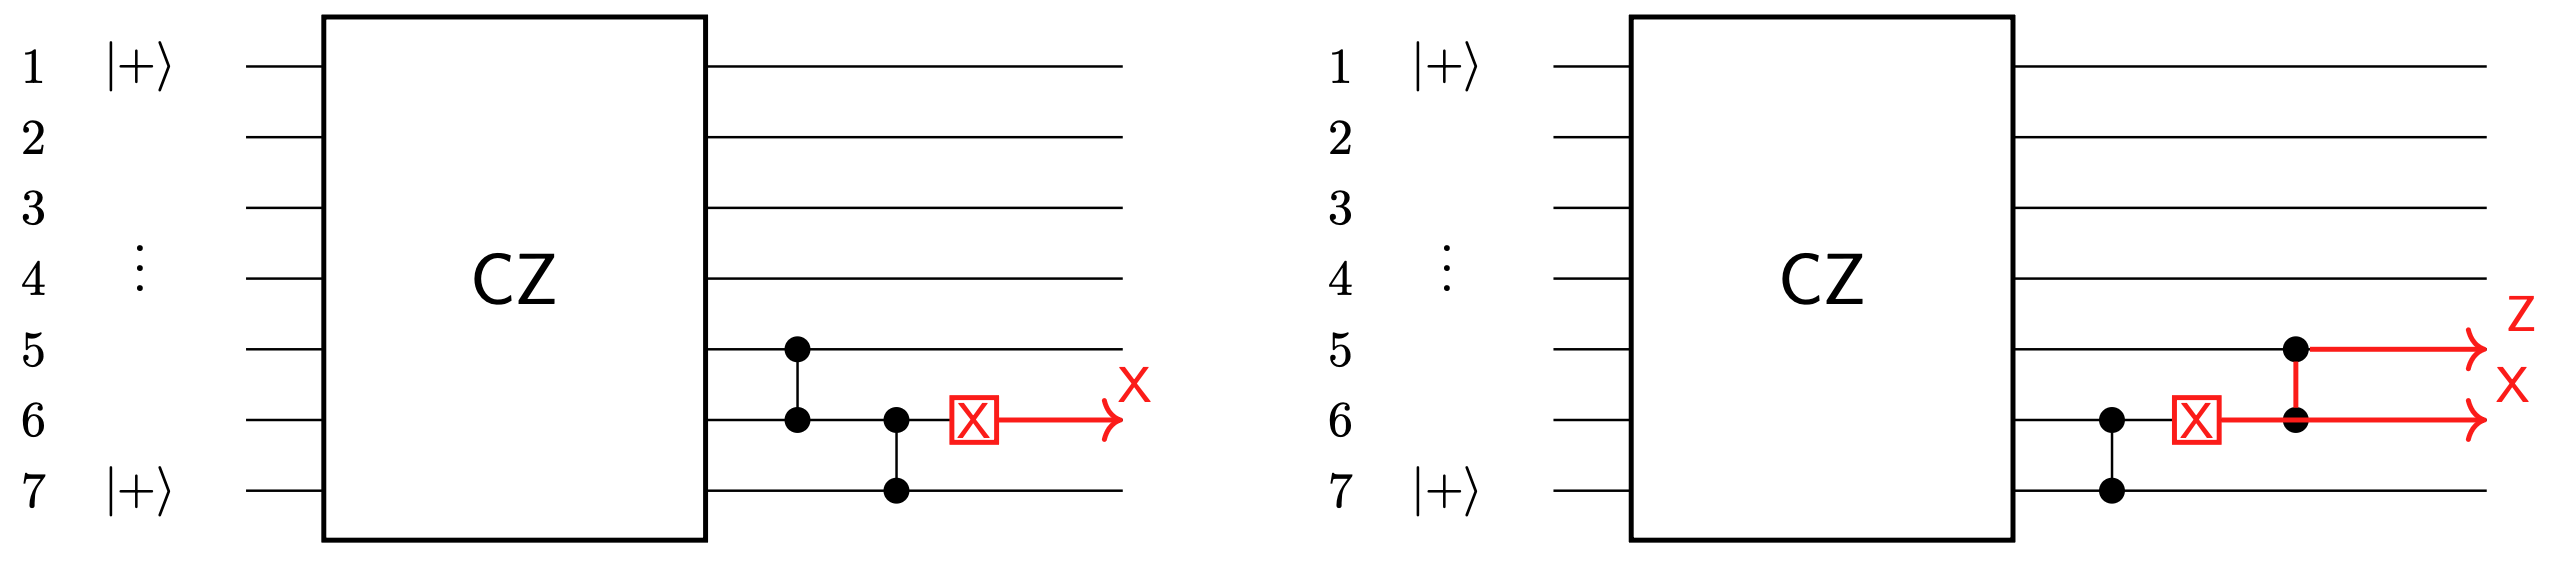
\includegraphics[scale=.32]{XZ.png}
\caption{Two gate orderings used to isolate depolarizing parameters associated with a central qubit. For an ordered triple $(5,6,7)$ with $(5,6),(6,7)\in E$, the relative order of $\CZ_{(5,6)}$ and $\CZ_{(6,7)}$ is swapped while keeping all other remaining gates fixed. Comparing the corresponding trap statistics yields equations that isolate the depolarizing strengths on the central qubit $6$ for the two incident edges.}
	\label{fig:orderings}
\end{figure}


\begin{figure}[H]
    \centering
    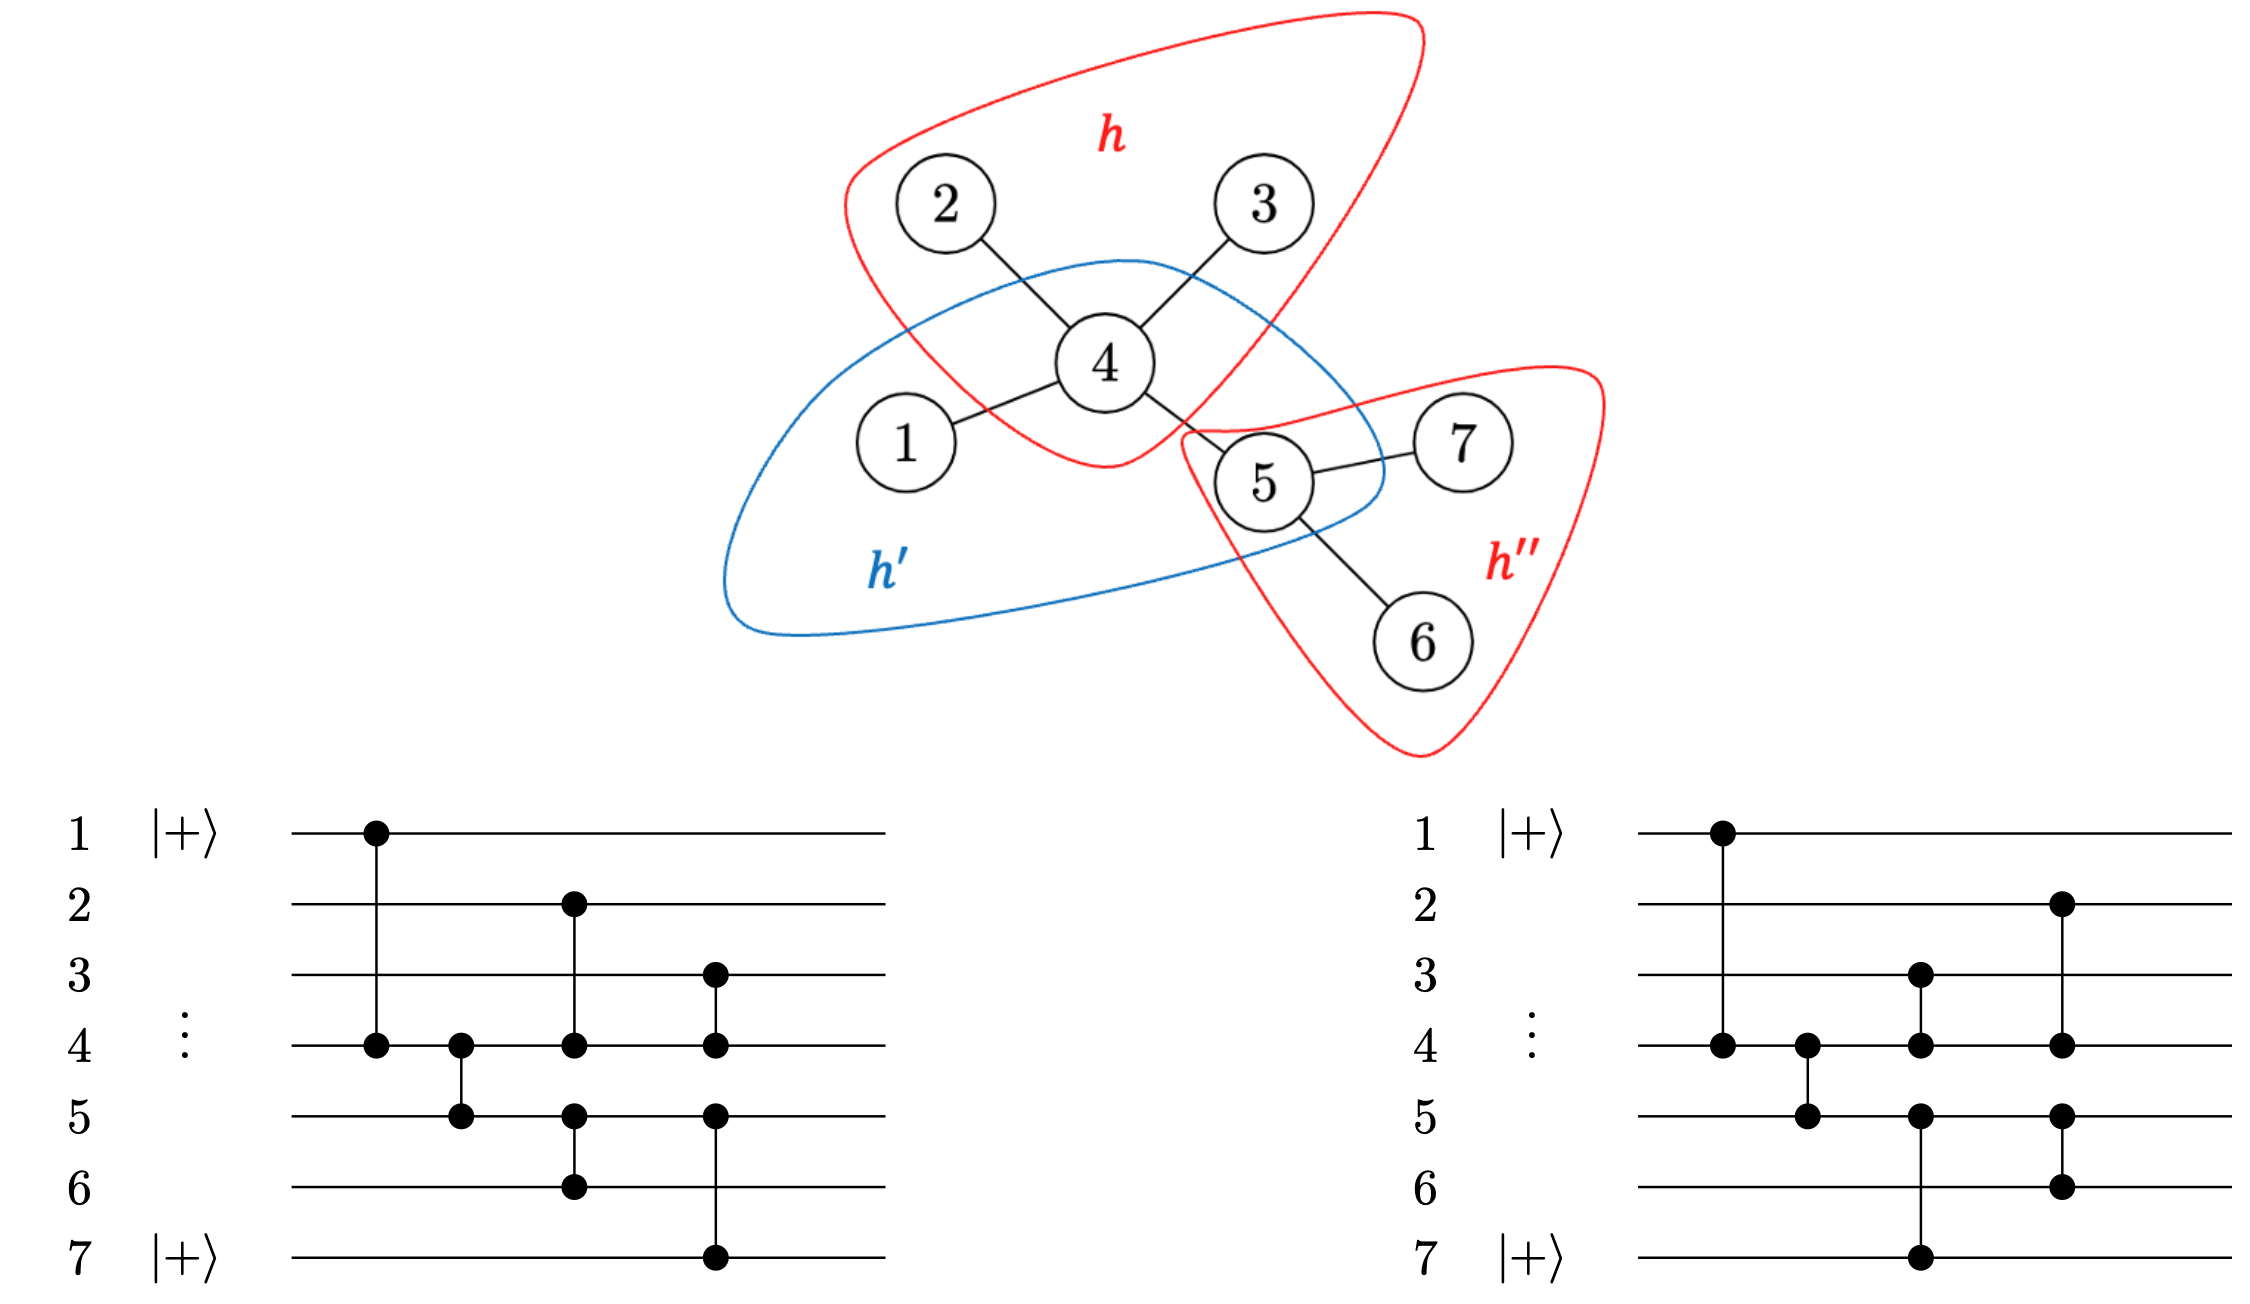
\includegraphics[scale=0.35]{singlecolor.png}
    \caption{Parallelizing the noise parameter estimation. (Top) Construction of the graph \(H\) from the edges of \(G\). An ordered triple, e.g.~\(h\), covers two adjacent edges in \(G\). These triples form the vertices \(W\) of \(H\). There is an edge in \(H\) between \(h\) and \(h'\) as they share vertices in \(G\). On the contrary \(h\) and \(h''\) are not connected by an edge in \(H\). As a consequence it is possible to fix the order of the \(\CZ\) gates corresponding to the edges covered by \(h\) and \(h''\) independently, which implies parallelization. (Left) and (Right) show how, in such situation, two orderings are enough to extract \(\lambda_{(2,4),4}, \lambda_{(3,4),4}, \lambda_{(5,6),5},  \lambda_{(5,7),5}\).}
	\label{fig:single-color-ordering}
\end{figure}


A minimization over the possible graphs \(H\) of the chromatic number would then give the minimum number of orderings for finding all depolarizing parameters. Yet, as finding the chromatic number of generic graphs is \textsf{NP-Hard}, so is this minimization in the general case. One can nonetheless work this out for specific graphs. For the 2D cluster state, one can construct \(H\) and show that its maximum degree is 7, which implies that the chromatic number is at most 8, and at most 16 orderings are enough (See \cref{fig:2d-cluster} for a possible construction of \(H\)).

A similar construction would also yield a graphical representation of conditions to parallelize the parameter estimation for cross-talk noise.

\begin{figure}[H]
    \centering
    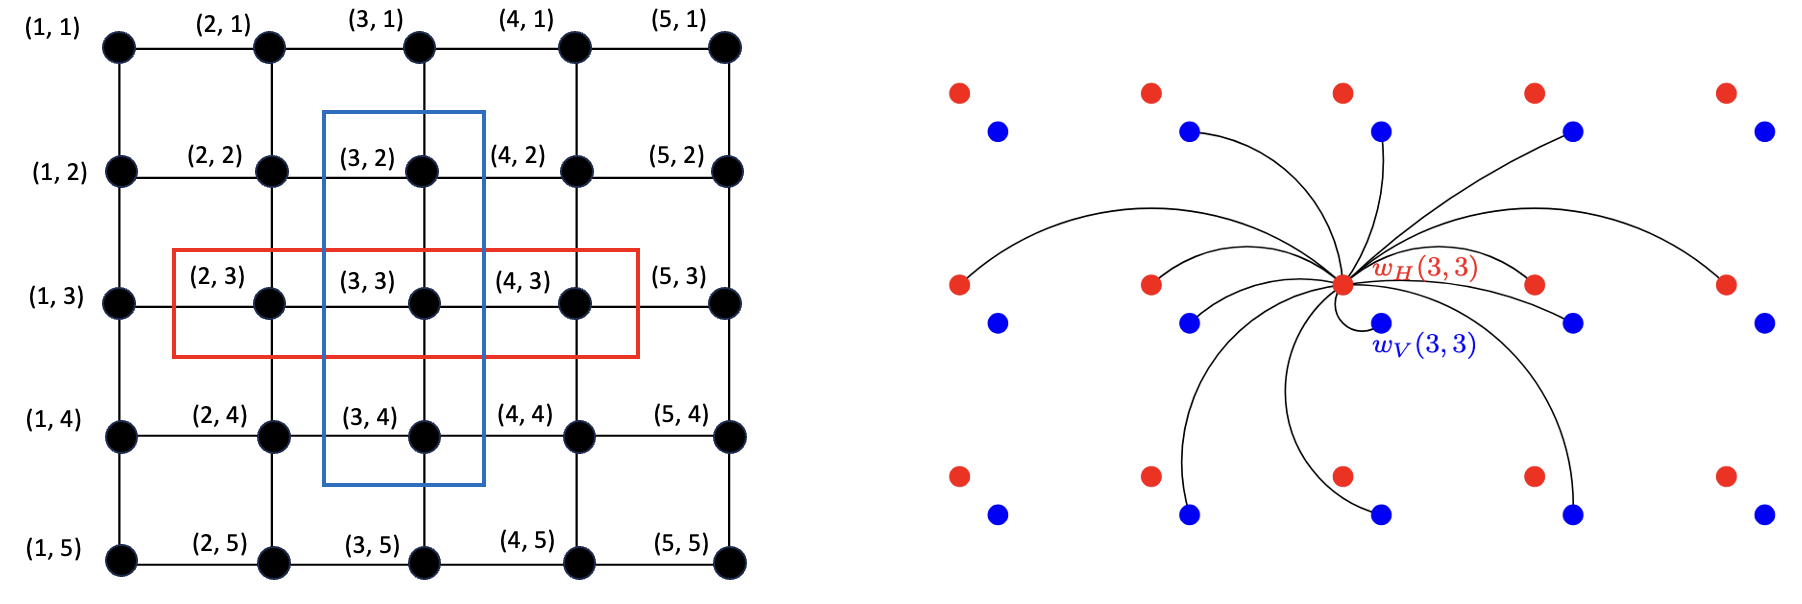
\includegraphics[width=1\linewidth]{cluster-conflict.png}
    % \caption{Example construction of the conflict graph $H$ for a 2D cluster state. Left: a $2\mathrm{D}$ cluster lattice with representative ordered triples centered at interior qubits (e.g., horizontal and vertical triples around $(3,3)$). Right: the local neighborhood of a representative vertex of $H$, showing that each triple conflicts with at most seven others in this construction. Hence $\Delta(H)\le 7$, implying $\chi(H)\le 8$ and therefore at most $2\chi(H)\le 16$ orderings are sufficient to recover all gate-level depolarizing parameters.}

%\input{local_h.pdf_t}

    \caption{Possible construction of the graph $H$ for a 2D cluster-state graph $G$.
      (Top) The black vertices and edges are that of the 2D cluster-state. Qubits are indexed by their coordinates on the grid. The blue and red sets of qubits are the two triples that need to be considered for constructing the graph \(H\) from \(G\) at qubit \((3,3)\). Indeed, at qubit \((3,3)\) there are four \(\lambda\) parameters to estimate, corresponding to the four edges incident to this qubit. Here, each triple infers two different parameters. This being the case for all qubits, the vertices in \(H\) can be partitioned in two sets corresponding to horizontal and vertical triples. ()Bottom) The graph \(H\) constructed around the horizontal triple of qubit \((3,3)\) denoted \(w_H(3,3)\). The vertex \(w_V(3,3)\) corresponds to the vertical triple for qubit \((3,3)\). The other red and blue nodes correspond to the horizontal and vertical triples for the qubits of the graph \(G\). The neighborhood of \(w_H(3,3)\) is made of all triples that share a qubit with it. This amounts to \(w_H(1,3), w_H(2,3), w_H(4,3), w_H(5,3)\) for the horizontal ones and \(w_V(2,2), w_V(2,3), w_V(2,4), w_V(3,2), w_V(3,3), w_V(3,4), w_V(4,2), w_V(4,3), w_V(4,4)\). This shows that the degree of \(w_H(3,3)\) is 13. By symmetry, with periodic boundary conditions on \(G\), all nodes in \(H\) have degree 13. This means that the chromatic number is bounded by 14 and that 28 orderings are enough to gather all possible depolarizing parameters for the 2D cluster state. Only the edges incident to $w_H(3,3)$ have been pictured.}
    \label{fig:2d-cluster}
\end{figure}


\paragraph{Beyond depolarizing channel.}
In the case where the noise is not depolarizing but still acts on each qubit independently, the strategy above would not work. The reason is that pure \(\Z\) noise commutes with the \(\CZ\) gates and its effect on traps does not depend on the orderings. As a result, it is impossible to split the source of \(\Z\) noise between the various gates acting on a given qubit. One possible way to bypass this limitation is to realize that one could instead selectively replace a given \(\CZ_e\) by \(\CZ_e \circ \CZ_e \circ \CZ_e\). This would accumulate the effect of the \(\Z\) noise and offer a way to estimate it for this specific gate. Similar ``tricks'' could be played to possibly extract information about even more complex noise models as long as their noiseless combined effect is the identity.

